\documentclass[12pt]{article}
\usepackage{geometry}                % See geometry.pdf to learn the layout options. There are lots.
\geometry{a4paper}                   % ... or a4paper or a5paper or ... 
%\geometry{landscape}                % Activate for for rotated page geometry
%\usepackage[parfill]{parskip}    % Activate to begin paragraphs with an empty line rather than an indent
\usepackage{graphicx}
\usepackage{amssymb}
\usepackage{epstopdf}
\DeclareGraphicsRule{.tif}{png}{.png}{`convert #1 `dirname #1`/`basename #1 .tif`.png}

\title{Review of basic frequentist concepts}
\author{Shravan Vasishth}
\date{25-29 March 2019}                                           % Activate to display a given date or no date

\begin{document}
\maketitle
%\section{}
%\subsection{}

\section{Foundations}

\subsection{Random variable}

A random variable $X$ is a function $X : S \rightarrow \mathbb{R}$ that associates to each outcome
$\omega \in S$ exactly one number $X(\omega) = x$.

$S_X$ is all the $x$'s (all the possible values of X, the support of X). I.e., $x \in S_X$. 

\textbf{Discrete example}: number of coin tosses till H

\begin{itemize}
  \item $X: \omega \rightarrow x$
  \item $\omega$: H, TH, TTH,\dots (infinite)
  \item $x=0,1,2,\dots; x \in S_X$
\end{itemize}

We will write $X(\omega)=x$:

$H \rightarrow 1$\newline

$TH \rightarrow 2$\newline

$\vdots$





The discrete binomial random variable X will be defined by

\begin{enumerate}
\item the function $X: S\rightarrow \mathbb{R}$, where S is the set of outcomes (i.e., outcomes are $\omega \in S$).
\item $X(\omega) = x$, and $S_X$ is the \textbf{support} of X (i.e., $x\in S_X$).
\item A PMF is defined for X:
\begin{equation}
p_X : S_X \rightarrow [0, 1] 
\end{equation}

\begin{equation}
p_X(x)= {n \choose x} \theta^x (1-\theta)^{n-x} 
\end{equation} 


\item A CDF is defined for X:
\begin{equation}
F(a)=\sum_{\hbox{all } x \leq a} p(x)
\end{equation}
\end{enumerate}

\textbf{Continuous example}: fixation durations in reading (the normal distribution)

\begin{itemize}
  \item $X: \omega \rightarrow x$
  \item $\omega$: 145.21, 352.43, 270, \dots 
  \item $x=145.21, 352.43, 270,\dots; x \in S_X$
\end{itemize}

The pdf of the normal distribution is:

\begin{equation}
f_{X}(x)=\frac{1}{\sqrt{2\pi \sigma^2}}
e^{-\frac{1}{2}\frac{(x-\mu)^{2}}{\sigma^2}},\quad -\infty < x < \infty
\end{equation}

We write $X\sim \mathtt{norm}(\mathtt{mean}=\mu,\,\mathtt{sd}=\sigma)$.

The associated $\texttt{R}$ function for the pdf is \texttt{dnorm(x, mean = 0, sd = 1)}, and the one for cdf is \texttt{pnorm}.

Note the default values for $\mu$ and $\sigma$ are 0 and 1 respectively. Note also that R defines the PDF in terms of $\mu$ and $\sigma$, not $\mu$ and $\sigma^2$ ($\sigma^2$ is the norm in statistics textbooks).


\begin{table}[!htbp]
\caption{Important R functions relating to random variables.}
\begin{center}
\begin{tabular}{|l|c|c|}
\hline
& Discrete & Continuous \\
\hline
Example: & Binomial(n,$\theta$) & Normal($\mu,\sigma$)\\
\hline
Likelihood fn & dbinom & dnorm \\ 
Prob X=x  & dbinom, pbinom & always 0 \\
Prob $X\geq x, X\leq x, x_1<X<x_2$   & pbinom & pnorm \\
Inverse cdf &  qbinom & qnorm \\
Generate fake data & rbinom & rnorm \\
\hline
\end{tabular}
\end{center}
\label{default}
\end{table}%

\subsection{Maximum likelihood estimate}

For the normal distribution, where $X \sim N(\mu,\sigma)$, we can get MLEs of $\mu$ and $\sigma$ by computing:

\begin{equation}
  \hat \mu = \frac{1}{n}\sum x_i = \bar{x}  
\end{equation}

and

\begin{equation}
	\hat \sigma ^2 = \frac{1}{n}\sum (x_i-\bar{x})^2
\end{equation}

you will sometimes see the ``unbiased'' estimate (and this is what R computes) but for large sample sizes the difference is not important:

\begin{equation}
  \hat \sigma ^2 = \frac{1}{n-1}\sum (x_i-\bar{x})^2
\end{equation}

The significance of these MLEs is that, having assumed a particular underlying pdf, we can estimate the (unknown) parameters (the mean and variance) of the distribution that generated our particular data. 

This leads us to the distributional properties of the mean \textbf{under repeated sampling}.

\subsection{The central limit theorem}

For large enough sample sizes, the sampling distribution of the means will be approximately normal, regardless of the underlying distribution (as long as this distribution has a mean and variance defined for it).

\begin{enumerate}
\item
So, from a sample of size $n$, and sd $\sigma$ or an MLE $\hat\sigma$, we can compute 

the standard deviation of the sampling distribution of the means.
\item We will call this standard deviation the estimated \textbf{standard error}.

$SE = \frac{\hat\sigma}{\sqrt{n}}$

I say \textit{estimated} because we are estimating SE using an an estimate of $\sigma$.

\end{enumerate}

The standard error allows us to define a so-called \textbf{95\% confidence interval}:

\begin{equation}
\hat\mu \pm 2 SE
\end{equation}

So, for the mean, we define a 95\% confidence interval as follows:

\begin{equation}
\hat\mu \pm 2 \frac{\hat\sigma}{\sqrt{n}}
\end{equation}

\textbf{What does the 95\% CI mean?}

\section{The t-test}

\subsection{The hypothesis test}

Suppose we have a random sample of size $n$, and the data come from a $N(\mu,\sigma)$ distribution. 

We can estimate sample mean $\bar{x}=\hat \mu$ and $\hat\sigma$, which in turn allows us to estimate the sampling distribution of the mean under (hypothetical) repeated sampling:

\begin{equation}
N(\bar{x},\frac{\hat \sigma}{\sqrt{n}})
\end{equation}

The NHST approach is to set up a null hypothesis that $\mu$ has some fixed value. For example:

\begin{equation}
H_0: \mu = 0
\end{equation}

This amounts to assuming that the true distribution of sample means is (approximately) normally distributed and centered around 0, \textit{with the standard error estimated from the data}.

The intuitive idea is that 

\begin{enumerate}
\item
if the sample mean $\bar{x}$ is near the hypothesized $\mu$ (here, 0), the data are (possibly) ``consistent with'' the null hypothesis distribution.
\item
if the sample mean $\bar{x}$ is far from the hypothesized $\mu$, the data are inconsistent with the null hypothesis distribution.
\end{enumerate}

We formalize ``near'' and ``far'' by determining how many standard errors the sample mean is from the hypothesized mean:

\begin{equation}
t \times SE = \bar{x} - \mu 
\end{equation}

This quantifies the distance of sample mean from $\mu$ in SE units.


So, given a sample and null hypothesis mean $\mu$, we can compute the quantity: 

\begin{equation}
t  = \frac{\bar{x} - \mu}{SE}
\end{equation}

We will call this the \textbf{observed t-value}.

The random varible T:

\begin{equation}
T  = \frac{\bar{X} - \mu}{SE}
\end{equation}

has a t-distribution, which is defined in terms of the sample size $n$. 
We will express this as: $T \sim t(n-1)$ 

Note also that, for large $n$, $T\sim N(0,1)$. 

Thus, given a sample size $n$, and given our null hypothesis, we can draw t-distribution corresponding to the null hypothesis distribution.

For large $n$, we could even use N(0,1), although it is traditional in psychology and linguistics to always use the t-distribution no matter how large $n$ is.

\subsection{The hypothesis testing procedure}

So, the null hypothesis testing procedure is:

\begin{enumerate}
\item Define the null hypothesis: for example, $H_0: \mu = 0$.
\item Given data of size $n$, estimate $\bar{x}$, standard deviation $s$, standard error $s/\sqrt{n}$.
\item Compute the t-value:

\begin{equation}
t=\frac{\bar{x}-\mu}{s/\sqrt{n}}
\end{equation}
\item Reject null hypothesis if t-value is large.
\end{enumerate}

\subsubsection{Rejection region}

So, for large sample sizes, if $\mid t\mid >2$ (approximately), we can reject the null hypothesis. 

For a smaller sample size $n$, you can compute the exact critical t-value:

\begin{verbatim}
qt(0.025,df=n-1)
\end{verbatim}

This is the critical t-value on the \textbf{left}-hand side of the t-distribution.
The corresponding value on the right-hand side is:

\begin{verbatim}
qt(0.975,df=n-1,lower.tail=FALSE)
\end{verbatim}

Their absolute values are of course identical (the distribution is symmetric).


Given iid data y:

\begin{verbatim}
t.test(y)
\end{verbatim}

Given two conditions' paired data vectors cond\_a, cond\_b (note that the order in which you write the vectors will determine the sign of the observed t-value):

\begin{verbatim}
t.test(cond_a,cond_b,paired=TRUE)
## identical to above:
t.test(cond_a-cond_b)
\end{verbatim}

Given data in long form, with the dependent variable written as y and the conditions marked by a column called cond:

\begin{verbatim}
t.test(y ~ cond,,paired=TRUE)
\end{verbatim}


\section{Type I, II error, power}

\begin{tabular}{ccc}
\hline
Reality: & $H_0$ TRUE & $H_0$ FALSE \\
\hline
Decision: `reject': & $\alpha$ & $1~-~\beta$ \\
                                     & \textbf{Type I error}                         & \textbf{Power} \\                                      
                                     & & \\
\hline
Decision: `fail to reject': & $1 - \alpha$ & $\beta$ \\                                    &                                 & \textbf{Type II error}\\
\hline
\end{tabular}

{\centering 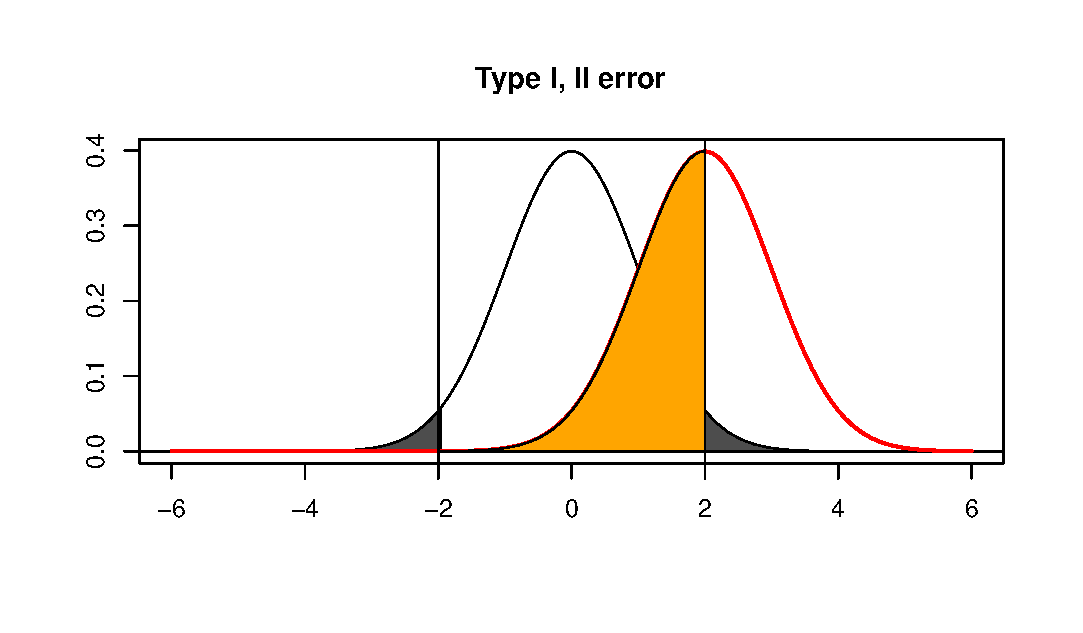
\includegraphics{figures/figure-unnamed-chunk-1-1} 
}


\section{Type M, S error}

If your true effect size is believed to be $D$, 
then we can compute (apart from statistical power) these error rates, which are defined as follows:

\begin{enumerate}
\item
\textbf{Type S error}: the probability that the sign of the effect is incorrect, given that the result is statistically significant.
\item 
\textbf{Type M error}: the expectation of the ratio of the absolute magnitude of the effect to the hypothesized true effect size, given that result is significant. 
Gelman and Carlin also call this the exaggeration ratio, which is perhaps more descriptive than ``Type M error''.
\end{enumerate}

{\centering 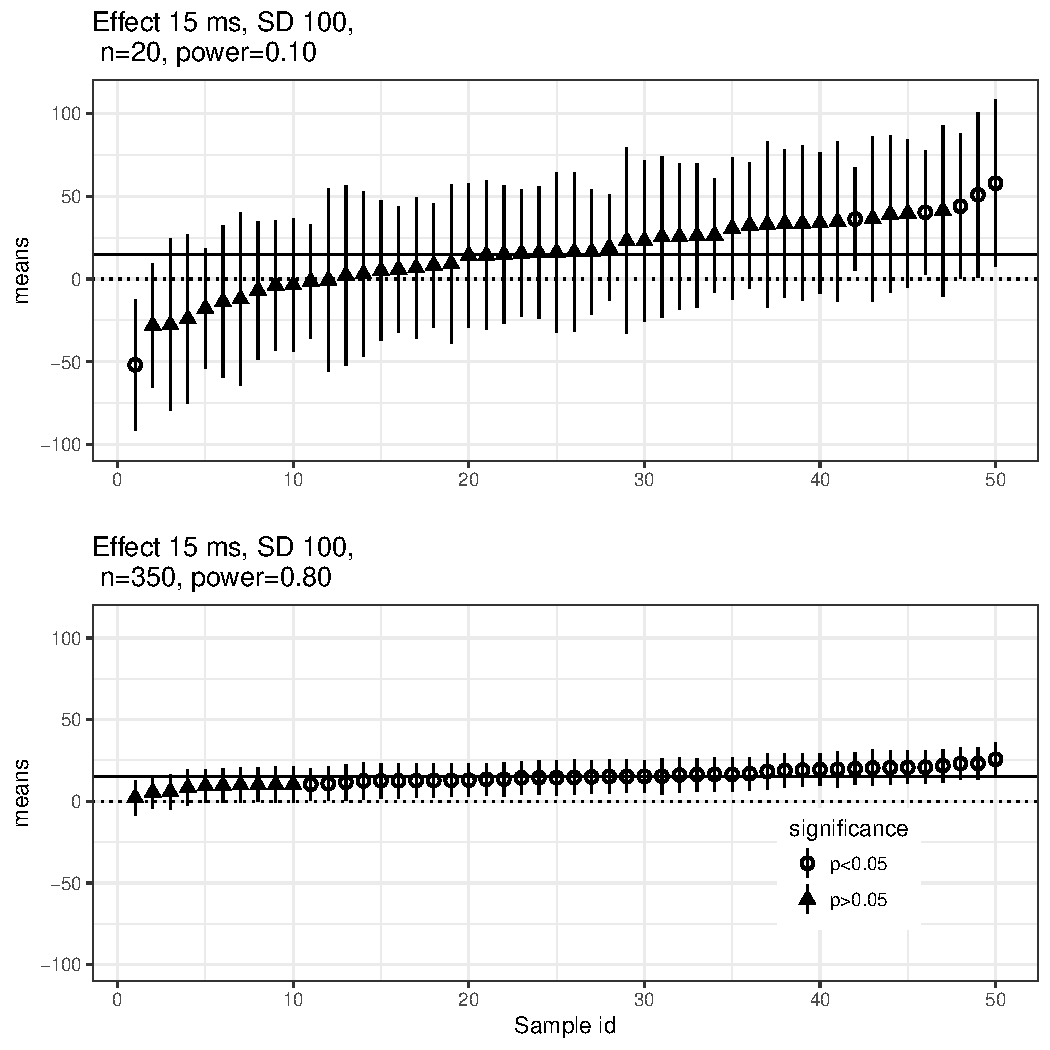
\includegraphics{figures/fig-demotypeM-1} 
}

\end{document}

\section{Linear models}

We consider the case where we have two conditions (e.g., subject and object relatives), and a repeated measures design. 

\subsection{Treatment contrast coding}

The alphabetically first condition level is coded 0, and the other condition level is coded 1. E.g., if condition labels are obj and subj, then obj is coded 0 and subj 1. You can change this with the command:

\begin{verbatim}
## code subj as 0 and obj as 1:
dat$condition<-factor(dat$condition,levels=c("subj","obj")
\end{verbatim}

In mathematical form, the linear model is:

\begin{equation}
rt = \beta_0 + \beta_1 condition + \epsilon
\end{equation}

where 

\begin{itemize}
\item
$\beta_0$ is the mean for the object relative
\item
$\beta_1$ is the amount by which the object relative mean must be 
changed to obtain the mean for the subject relative.
\end{itemize}

The null hypothesis is that the difference in means between the two relative clause types $\beta_1$ is:

$H_0: \beta_1 = 0$

We will make a distinction between the \textbf{unknown true mean} $\beta_0, \beta_1$ and the \textbf{estimated mean from the data} $\hat\beta_0, \hat\beta_1$.
From the example in the slides:

\begin{itemize}
\item
Estimated mean object relative processing time: $\hat\beta_0=471$
.
\item
Estimated mean subject relative processing time: $\hat\beta_0+\hat\beta_1=471+-102=369$.
\end{itemize}

\subsection{Sum contrast coding}

We can code obj as +1 and subj as -1 (or vice versa). Then:

\begin{itemize}
\item
Estimated \textbf{grand mean} processing time: $\hat \beta_0=420$.
\item
Estimated mean object relative processing time: $\hat\beta_0+\hat\beta_1=420+51=471$.
\item
Estimated mean subject relative processing time: $\hat\beta_0-\hat\beta_1=420-51=369$.
\end{itemize}

This kind of parameterization is called \textbf{sum-to-zero contrast} or more simply \textbf{sum contrast} coding. This is the coding we will use.

The null hypothesis for the slope is

\begin{equation}
H_0: \mathbf{1\times} \mu_{obj} + (\mathbf{-1\times}) \mu_{subj} = 0   
\end{equation}

The sum contrasts are referring to the $\pm 1$ terms in the null hypothesis:

\begin{itemize}
\item object relative: +1
\item subject relative: -1
\end{itemize}

the model is:

Object relative reading times:

\begin{equation}
rt = 420\mathbf{\times 1} + 51\mathbf{\times 1} + \epsilon
\end{equation}

Subject relative reading times:

\begin{equation}
rt = 420\mathbf{\times 1} + 51\mathbf{\times -1} + \epsilon
\end{equation}

\subsection{Normality assumption of the residuals in the linear models}

The model is:

\begin{equation}
rt = \beta_0 + \beta_1 + \epsilon \hbox{ where }  \epsilon\sim Normal(0,\sigma)
\end{equation}

It is an assumption of the linear model that the residuals are (approximately) normally distributed.

We can check this assumption in R. For a full and formal review of linear models (including linear mixed modeling), see: https://github.com/vasishth/LM

\end{document}  